\chapter{The Architecture of the SAFE Network}
\label{ch:architecture}

The internet is constantly growing and changing. Changes in technologies slowly permeate throughout the network as if by osmosis. Governmental policy can have a large impact on how people interact with the network, whether that be Turkey blocking Wikipedia\cite{turkey} or the US abandoning Net Neutrality. This area is where the SAFE Network starts to deviate greatly from the \textit{traditional} internet. The SAFE Network is a ``Autonomous Data Network''. To have access to the SAFE Network means to have access to all of it. A government cannot curate access data. This is made possible by the architecture of the SAFE Network.

\section{Vaults and Clients}

The SAFE Network is comprised of \textit{vaults}. A \textit{vault} is a singular program/application that a user runs on their computer, whether that be a server hosted in a datacenter or a desktop computer. A \textit{vault} is given a set amount of storage by the user which it then uses to \textit{farm} data. For a given \textit{vault} to join the network, it must pass a ``Proof of Resource'' test. This test is used to validate that the \textit{vault} has enough bandwidth and CPU power to be able to adequately perform its job. Similar to how a real world farmer looks after their crop/animals, a \textit{farmer} (\textit{vault}) on the SAFE Network looks after data. Understanding that nomenclature is quite useful in understanding the function a \textit{farmer} (\textit{vault}) serves. When a \textit{vault} successfully serves the data it is storing, it is rewarded with \textit{Safecoin}. A cryptocurrency hosted on the SAFE Network. Reading data from the network doesn't incur any cost, it is only when writing data that a user (\textit{client}) has to expend \textit{Safecoin}. A user doesn't need to run their own \textit{vault} to interact with the network, all users can connect through the use of a lightweight \textit{client}.

The only time a user interacts with their \textit{vault} is through configuration before startup. The most notable configuration being the allocation of storage for the \textit{vault} to use. Once \textit{vaults} start communicating with each other, humans have no control over their operation. The network autonomously votes and decides many factors which includes everything from where data should be stored to how much value a single \textit{Safecoin} has. This is the autonomy of the network, it does not accept governance by humans and \textit{vaults} cooperate for the good of the entire network.

\section{Immutable and Mutable Data}

Similar to BitTorrent, data is broken down into chunks. Each chunk of data that is stored on the SAFE Network is at most 1MB in size and has a unique 256-Bit Address. This allows every chunk of data to be uniquely identified and helps \textit{vaults} to decide who stores the data. Data stored on the SAFE Network can take one of two forms. It can either be \textit{Immutable Data} or \textit{Mutable Data}. A Mutable Data structure is a \textit{key value} storage mechanism that allows for the storage of one thousand entries. An Immutable Data structure only stores a single ``value'', its address derived from the hash of the binary data it contains. An Immutable Data structure can itself only be 1MB in size, but through the use of a \textit{data map} (Section \ref{subsec:self-encryption-data-map}) this limit can be subverted. As their names imply, Mutable Data can be freely mutated whereas Immutable Data cannot. It is this property of Immutable Data that eliminates duplication on the network. For example, if Bob uploads a picture to the network he is presented with the address of that file (the address of a \textit{data map}) and will have the relevant keys to access it. If Alice then uploads the exact same picture the data is not duplicated, she is simply presented with another \textit{data map} to the data. If either Bob or Alice chooses to ``delete'' the picture, then they simply ``forget'' how to access their \textit{data map}. This means that if someone has access to a piece of data then that ability will never be revoked.

\subsection{Self Encryption and Data Maps}
\label{subsec:self-encryption-data-map}

\begin{figure}[h]
	\begin{center}
		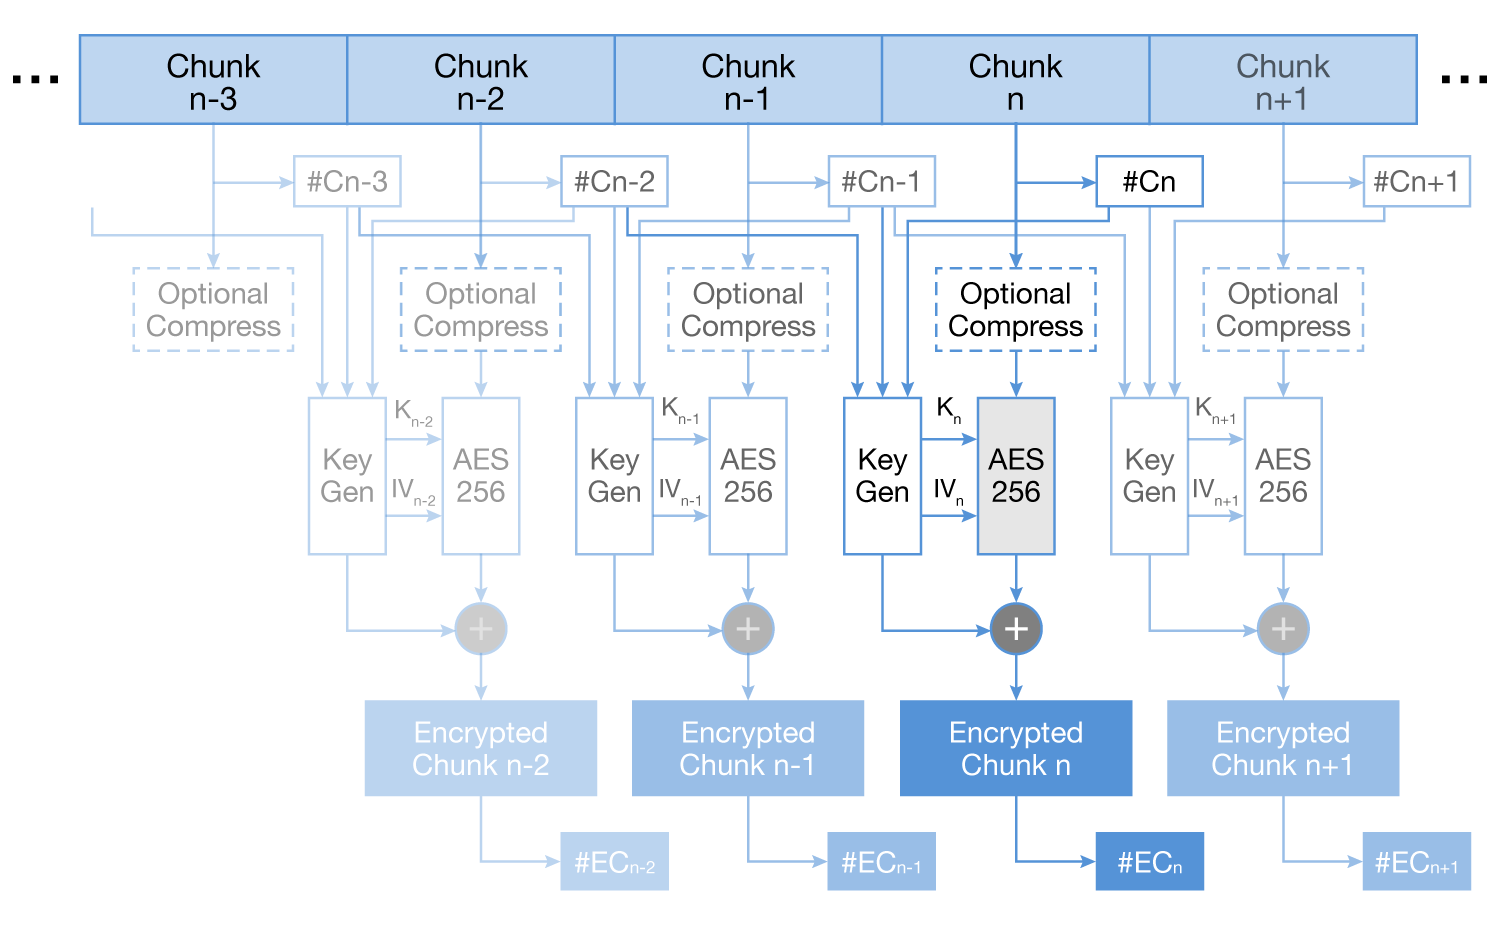
\includegraphics[width=\textwidth]{diagrams/self-encryption}
		\caption{The \textit{Self Encryption} process \protect\footnotemark}
		\label{fig:self-encryption}
	\end{center}
\end{figure}

\footnotetext{Sourced from https://safenetwork.wiki/en/Encrypt}

Immutable Data that is stored on the SAFE Network goes through a process called \textit{Self-Encryption}\cite{irvine2010self}. During \textit{self-encryption} data is broken down into chunks of a specified size (The SAFE Network uses 1MB chunks). To be able to reassemble and read the data a structure known as a \textit{data map} is created during the process. The \textit{data map} contains several pieces of information:

\begin{itemize}
	\item chunk\_num u32: Specifies how many chunks of data are within the Data Map
	\item hash Vec\textless u8\textgreater: Post-encryption hash of chunks
	\item pre\_hash Vec\textless u8\textgreater: Pre-encryption hash of chunks
	\item source\_size u64: The size of the original piece of data, before any encryption has taken place
\end{itemize}

The crucial structures of this \textit{data map} are the two vectors that store the pre-encryption and post-encryption hashes of chunks. What happens first is a piece of data is broken down into chunks and then hashed. The hash of the chunks is stored in the `pre\_hash Vec\textless u8\textgreater' of the \textit{data map}. This list is important as it defines the original piece of data before being encrypted. Each chunk then goes through an encryption process using AES 256. The key used for each chunk is the pre-encryption hash of one of the other chunks. The chunks then go through another step that further obfuscates the data. This step involves XOR'ing the data with the pre-encryption hash of other chunks. A final hash is then taken of each chunk and stored in the `hash Vec\textless u8\textgreater' of the \textit{data map}. A diagram illustrating \textit{self-encryption} can be seen in Figure \ref{fig:self-encryption}.

\textit{Self-Encryption} is a generic process, there is nothing about it that specifically ties it to the SAFE Network. \textit{Self-Encryption} is used to obfuscate data for storage, it is only with access to the \textit{data map} that you can make sense of the data. It is because of this obfuscation process that \textit{vaults} cannot distinguish what the chunks they are storing actually contain. It is just ``garbage'' data to them. This means chunks can be freely distributed across the network with the assurance that only the person with access to the \textit{data map} can read the original data. To secure access to the \textit{data map} it can be encrypted using either a symmetric key or an asymmetric key-pair. With different key-exchange mechanisms users can then freely share access to \textit{data maps} with one another.

\subsection{Address Collision}
\label{subsec:address-collision}

The SAFE Network stores chunks based on 256-Bit addresses. Although the probabilities are unfathomably small, collisions in the post-encryption hash of chunks from \textit{self-encryption} is possible. The hash algorithm used currently is \textit{SHA3-256}\cite{dworkin2015sha} which was first published in 2015. \textit{SHA3-256} is an incredibly ``safe'' hashing algorithm to use, papers like \citetitle{amy2016estimating}\cite{amy2016estimating} do propose methods on how to ``break'' the algorithm but their findings indicate that even with Quantum computers an attack would be practically unfeasible. The question as to why use \textit{SHA3-256} when stronger algorithms exist within the same family is however curious. NIST themselves currently recommend\cite{hash-reccomend} that for generic hashing applications \textit{SHA3-512} is the minimum algorithm that should be used. This brings into question why Maidsafe have chosen a less secure algorithm. If the choice came down to performance then this is an oversight that could hurt them in the long run. Moore's law\cite{schaller1997moore} says that as time passes computers become more and more capable. If the SAFE Network truly wants to exist for a long period of time, choosing \textit{SHA3-256} as the hashing algorithm the entire network is based upon seams like a naive approach. The suggestion to use the strongest algorithm that exists today is thus highly encouraged, a switch to \textit{SHA3-512} seams like a logical step. Especially given the fact that currently the network doesn't handle hash collisions, it simply writes over any collisions that occur.

\subsection{True Immutability of Data}
\label{subsec:immutability-of-data}

Once Immutable Data has been written to the network it can never be changed or deleted. The chunks of data that are the result of \textit{self-encryption} will be stored by the network indefinitely. This means that to ``delete'' data more accurately means to ``forget how to access it''. The implication of this is that once data is uploaded, access to the \textit{data map} is the only thing that stands between being able to access the data and it being lost forever. Not having any mechanism to actually delete data does pose problems.

\subsection{Mutable Data}

A Mutable Data Structure facilitates a powerful ``permission scheme'' to data and is controlled by the user who creates it. Unlike Immutable Data, the address of Mutable Data doesn't have to correspond to a hash. For Immutable Data, the location of the ``data'' is actually the address of the chunk that contains the \textit{data map}. The hash of the original file is the address of that chunk. There is no such limit on Mutable Data and hence can be stored at any empty address. As the name implies, the special thing about Mutable Data is that it can be mutated.

The permission scheme around MD is what gives it its utility. The ``owner'' of the MD can specify exactly who can perform what actions to the MD structure. The generic actions that can be performed are: insert, update, delete and change permissions. To give an example, a user could have an email address on the network that has an ``inbox'' MD structure. Everyone would then be granted the permission to ``insert'' to the MD, all other permissions would only be granted to its ``owner''. Using asymmetric encryption they could then encrypt the ``inserts'' to the structure so that only the ``owner'' of the MD is able to read the entries. As MD structures don't need to live in a chunk thats address corresponds to the hash of the chunk, they can be at custom locations. So to find the ``inbox'' for someone is as simple as taking the SHA3-256 hash of their username/email-address and then ``inserting'' messages to the corresponding MD.

It is this permission scheme that allows complex and dynamic applications to be built whilst giving users the ability to still control their ``own'' data.  As MD structures can be mutated, they can be used to direct clients towards files that are Immutable Data. For instance, if a user visits a website the MD that points to the HTML, CSS, etc, can be found at the SHA3-256 of the URL. As it is a MD the ``owners'' of the website can simply update this index to point to newer revisions of the website files when they wish to update the website.

\section{Disjoint Sections}

The unique address of every 1MB chunk of data is used to determine what \textit{vaults} are responsible for storing it. Maidsafe's innovation was in the creation of what are called \textit{Disjoint Sections}. These \textit{sections} are groups of \textit{vaults} that are responsible for a certain range of the 256-Bit address space. By default, the network requires a minimum number of \textit{vaults} to sustain the network. At the time of writing this is eight \textit{vaults}. These eight \textit{vaults} form a complete \textit{section} and are responsible for the storage of the entire 256-Bit address range. As more \textit{vaults} join the network, this \textit{section} will grow in size and then eventually split into two new \textit{sections}. There are numerous requirements that have to be met before a \textit{section split} is allowed.

\begin{figure}
	\begin{center}
		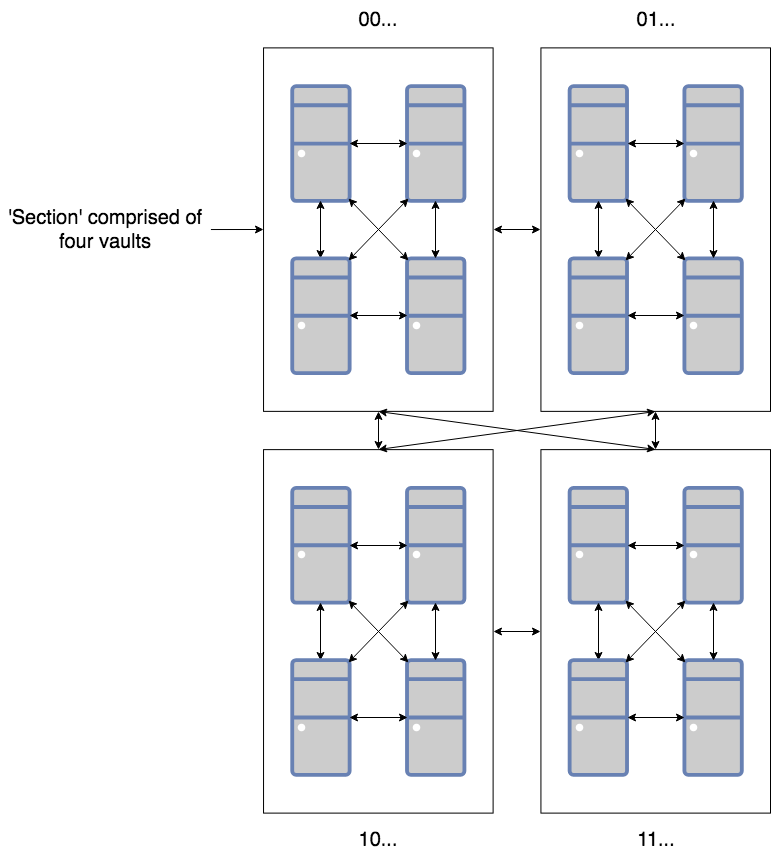
\includegraphics[scale=0.3]{diagrams/safe-network-sections}
		\caption{Four sections of a SAFE Network. You can see the address range each section is responsible for.}
		\label{fig:safe-sections}
	\end{center}
\end{figure}

After a split, \textit{sections} are then responsible for half of the 256-Bit address range that they were before. As more complete \textit{groups} of ~eight \textit{vaults} join the network, it continues to split and each \textit{section} is therefore responsible for less data. An important thing to note is that the SAFE Network doesn't assign 256-Bit addresses based on proximity. In a given \textit{section} two \textit{vaults} could be located on different continents. This property helps the integrity of the network by ensuring \textit{vaults} in a given \textit{section} are not located close to one another. Otherwise the network could be open to simple attacks. For example, start eight \textit{vaults} on a single computer to form a \textit{section} then switch them all off. The loss of an entire \textit{section} could result in data loss. If a significant number of \textit{vaults} leave the network then \textit{sections} have the ability to merge with other \textit{sections} to ensure the stability of data is maintained. In Figure \ref{fig:safe-sections} four \textit{sections} comprised of four \textit{vaults} can be seen, the address range that each \textit{section} is responsible for can be seen beside them. In the diagram four \textit{vaults} make a \textit{section} instead of the traditional eight, this is just to make the diagram easier to process.

\section{Proof of Resource}
\label{subsec:proof-of-resource}

The \textit{proof of resource} (PoR) test is used to validate the effectiveness of a \textit{vaults} ability to store and serve data. PoR is used during certain events, such as a \textit{vault} joining the network, to validate that it can adequately perform its job. \textit{Vaults} will further be asked to perform a PoR during random network events, this means that \textit{vaults} are continually tested to check that they haven't lost the ability to serve the network.

\section{Personas}

\textit{Vaults} can be characterised as having different \textit{personas}. One such \textit{persona} is the \textit{Data Manager}. A \textit{Data Manager} is responsible for the curation of data chunks within a given \textit{section}. When data is stored on the network, it is replicated across multiple \textit{Data Managers} in a \textit{section}. At all times the network aims to keep a minimum number of copies of a chunk of data, if a copy goes missing then it is replicated to a \textit{Data Manager} to ensure that data is stored redundantly. Hence within a given section, there will be several \textit{vaults} storing identical chunks of data. Each having full knowledge of the chunks of data that the other \textit{Data Manager's} hold. This scheme means that no \textit{vault} will ever hold the single copy of a chunk of data.

Another important \textit{persona} is that of the \textit{Client Manager}. A \textit{Client Manager} is responsible for storing the account data for clients that fall within its address space. It is also responsible for liaising with the rest of the network on behalf of that account. When a user creates an account on the SAFE Network the data is stored on the network just like any other piece of data. It has a given 256-Bit address and contains information like: how much \textit{Safecoin} it has, the number of chunks of data that has been uploaded, etc.

\section{Accounts}

Accounts on the SAFE Network are not inherently special in that they are stored along with other pieces of data on the network. There is no centralised body or organisation that is needed to grant access to the network. An account on the SAFE Network is derived from two parts, an \textit{Account Secret} and a \textit{Account Password}. The \textit{Account Secret} identifies where the account is stored then the \textit{Account Password} is used to encrypt and decrypt that information. With these two components a user can gain access to a piece of data that represents their account. This data structure contains everything needed for an account:

\begin{itemize}
	\item The Safecoin balance of the account
	\item Address(es) of \textit{data maps} that the account has decryption keys for
	\item Decryption keys for the aforementioned \textit{data maps}
	\item Other account information
\end{itemize}
	
An important caveat that comes from having a single set of credentials is that once lost, a user cannot access their account again. This is not a real problem for ``professional'' users as most make use of password managers and other such tools. At some point though even the most ``pro'' user could lose track of a password and with that their data is gone. There is no chance of recovery. This could involve losing irreplaceable data which can be heart-breaking for individuals and bankruptcy causing for companies. Thus keeping credentials safe is extremely important. This could be a prohibiting factor to a lot of users however, some may not want to take the risk.
\section{Crust and Encryption}

\textit{Crust} is the secure routing layer designed and built by Maidsafe to provide the secure communications backbone of the SAFE Network. \textit{Crust} allows for reliable P2P connections and provides encryption for all traffic. Several transmission protocols can be used, falling back to UDP from TCP (for example) if required. Encryption at this level means that data in transit is always encrypted, no matter what.

\begin{figure}
	\begin{center}
		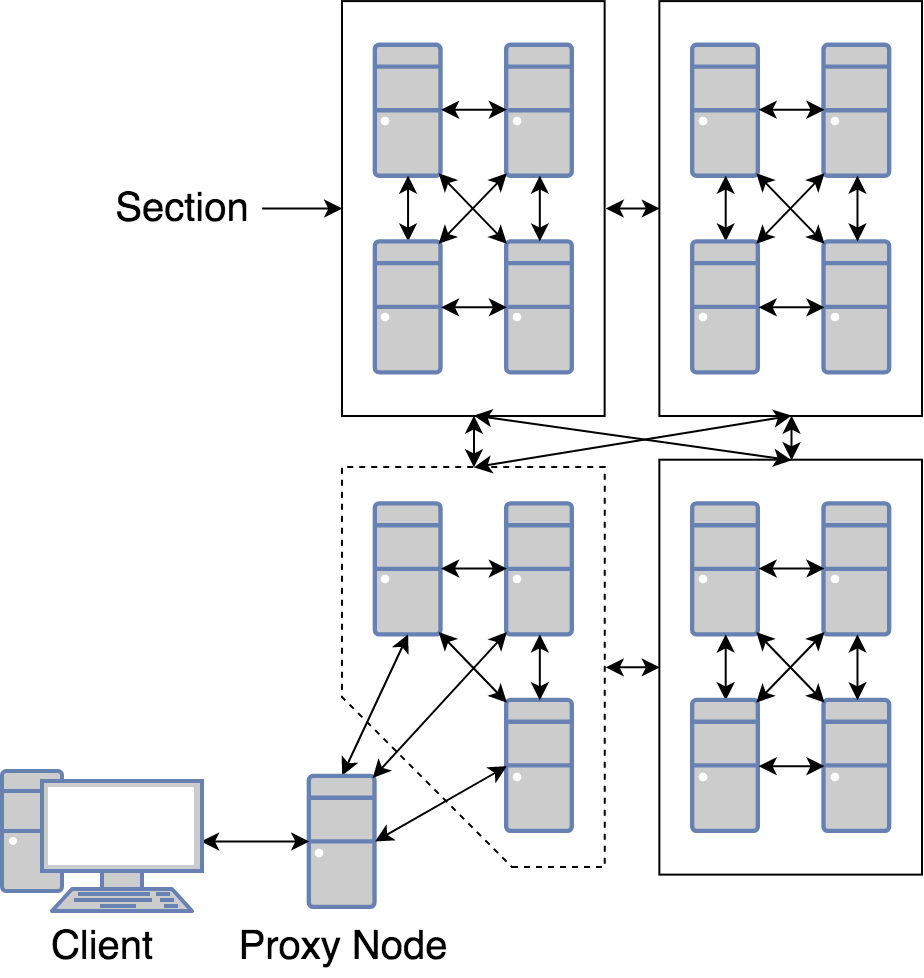
\includegraphics[scale=0.3]{diagrams/safe-network-connection}
		\caption{A client connecting to the SAFE Network through a Proxy Node}
		\label{fig:proxy-connection}
	\end{center}
\end{figure}

When a client connects to the network they do so through the use of a \textit{Proxy Node}. A \textit{proxy node} is a \textit{vault} that is used to liaise between a client and the network at large. The \textit{proxy node} is used to hide the clients IP address from the rest of the network. Deeper into the network, \textit{vaults} communicate directly with this \textit{proxy node} and not with client. Hence through the use of a \textit{proxy node}, the real world identity of the client is well hidden from the rest of the network. This means that a given \textit{vault} cannot detect that the data it is sending is going to a certain geographical location. The topology of how a client connects to the SAFE Network can be seen in Figure \ref{fig:proxy-connection}.

\section{Network Incentives, Safecoin and Farming}

\textit{Safecoin}\cite{lambert2015safecoin} is the cryptocurrency of the SAFE Network. When a user creates an account on the network, they are given a \textit{Safecoin} wallet. This wallet can be used to securely store the \textit{Safecoin} that belongs to the account. Akin to \textit{Bitcoin}, \textit{Safecoin} is a cryptocurrency that can be sent between users in a permission-less manner. \textit{Safecoin} can be sourced in a number of ways including through \textit{farming} and by simply purchasing them with another currency. The ultimate purpose of \textit{Safecoin} is to incentivise people to run \textit{vaults}. Running a \textit{vault} is costly, so the reward of \textit{Safecoin} is used to incentivise the participation of nodes in the network. The expectation is that as the cost of CPU/storage falls with time, the value of \textit{Safecoin} will increase. Value in this context is how much data each coin facilitates the storage of.

When a client requests a chunk of data, the \textit{vault} that successfully returns that piece of data will be given the opportunity to earn \textit{Safecoin}. The probability of being awarded this attempt to earn \textit{Safecoin} is determined by the \textit{farming rate} of the network at that specific moment in time. The \textit{farming rate} is used to balance supply and demand of data on the network. The SAFE Network tries at all times to keep a minimum amount of network capacity free, this is around \%30. When capacity starts to fall below this threshold then the \textit{farming rate} will increase, meaning \textit{vaults} have the opportunity to earn more \textit{Safecoin}. This works in the opposite direction too. If the network grows so that there is an overabundance of capacity then the \textit{farming rate} will decrease meaning \textit{vaults} earn less money. This constantly varying \textit{farming rate} is hence used to balance network resources and de-incentivise users from starting new \textit{vaults} when they are not needed.

The utility of \textit{Safecoin} is not tied to whatever its ``exchange price'' is. Overtime, the storage ``buying power'' of each \textit{Safecoin} should increase as computing power and storage becomes cheaper. \textit{Safecoin} is in its infancy and indeed has not yet been implemented, which means it is subject to changes from what has been described above.

\section{Quorum and the Datachain}
\label{sec:datachain}

As the network acts as an autonomous entity there has to be some method for a given \textit{vault} to reach consensus with other \textit{vaults}. This problem is what cryptocurrencies aim to solve through processes such as mining. \textit{Mining} is essentially the network reaching consensus upon what has happened. In the case of \textit{Bitcoin}, every time a block is \textit{mined} it is cryptographically linked to the block that came before it. As this \textit{Blockchain} grows in size the consensus on past transactions becomes stronger. The SAFE Network needs a similar mechanism on how to reach consensus. Analogous to a \textit{Blockchain}, the SAFE Network has a \textit{Datachain}.

The Datachain is used to help insure the integrity of the network and can be used to help rebuild it in the case of a catastrophic failure. For any action on the network to be valid, whether this be the storing/mutation of data or a \textit{vault} joining a \textit{section}, there has to be a corresponding \textit{group signature}. This \textit{group signature} is stored in the \textit{Datachain} that all \textit{vaults} in a \textit{section} have. In order for an action to be considered valid, a \textit{section} has to reach a quorum. For a network where the minimum \textit{section} size is eight, a quorum would be five out of the eight vaults voting in agreement. This means that in a given \textit{section}, several \textit{vaults} could be acting as ``bad parties'' but network integrity wouldn't be lost. The closer two \textit{sections} are in 256-Bit XOR address space the more they know about the data the other is storing. They will have access to the portion of the \textit{Datachain} that is used by that \textit{section} to record data writes and mutations. This way a given \textit{section} can help to verify that a neighbour is acting as a ``good party'' and that data being stored there has not been tampered with. The further away two \textit{sections} are in 256-Bit address space the less they know about each other. This means that as the number of \textit{sections} increases, the influence a given \textit{section} has over the network decreases. Eventually resulting in no \textit{section} having a complete overview of the entire network.

A protection mechanism exists for when a \textit{vault} tampers with data after it has been recored in the \textit{Datachain}. When a client requests a given piece of data, a single \textit{vault} is chosen to return that chunk of data. Alongside the data that is returned, a number of acknowledgements from other \textit{vaults} in the \textit{section} must be returned too. This way, a client can then verify the data they receive against the acknowledgements from the other \textit{vaults} in order to ensure that the data is valid.

The development of the \textit{Datachain} is still very active, thus implementation details are subject to rapid change.

\subsection{Node Age and Churn}

For a \textit{vault} to vote on network activity it has to have proven itself reliable. A \textit{vault} cannot just join the network and start voting in network decisions. When a new \textit{vault} announces itself to the network, it is issued with the POR test that was discussed in Section \ref{subsec:proof-of-resource}. If it passes then as long as the assigned \textit{section} reaches a quorum the \textit{vault} will join that \textit{section} and it will be recorded in the \textit{Datachain}. The new \textit{vault} is very ``young'' in the eyes of the network and as such cannot be trusted. It is not allowed to vote in group actions and is responsible only for the storage and transmission of data.

\textit{Churn} is used to continuously ``rotate'' vaults round different \textit{sections} on the network. This means that in a given time frame, a \textit{vault} will not be responsible for the same 256-Bit address range. This important feature helps to ensure that it is very difficult to track down where data is stored in order to erase it or corrupt it. During \textit{churn}, young \textit{vaults} with a lower \textit{node age} will be chosen more frequently than older \textit{vaults}. The \textit{vaults} chosen are assigned to new \textit{sections} to which they must provide another PoR test to be allowed to join. If the new \textit{section} reaches a quorum then the \textit{vault} joins and its \textit{node age} is incremented. Thus, trust must be earned by acting as a ``good party'' in the network over time. Only when a \textit{vault} reaches a certain \textit{node age} does it become an \textit{elder}. An \textit{elder} is a node which has the highest possible \textit{node age}, meaning it has has proven itself to be a reliable party over the course of time. When a \textit{vault} is an \textit{elder}, it gains the voting rights that lead to the construction and maintenance of the \textit{Datachain}. If a \textit{vault} acts out of order then its \textit{node age} can be decremented or eliminated entirely. Trust must be earned.

\textit{Node ageing} and \textit{churn} are hence essential security features of the network and make it very difficult for an attacker to have any choice in the \textit{section} of the network they wish to attack.

\section{Opportunistic Caching}

If a \textit{vault} is involved in the routing of a chunk of data that it sees frequently, it has the ability to cache that chunk. Owing to the architecture of the SAFE Network, content cannot ``go down'' due to high traffic. The network will respond autonomously to the higher volume of traffic and dynamically increase its potential to serve that content.
 
 Another benefit of this caching is geographical proximity. A good example is that of a website that has support for multiple languages. Due to caching, chunks that correspond to particular languages will be cached in the \textit{vaults} nearest to where they are being consumed. For instance, the chunks that correspond to Japanese content will more likely be cached in \textit{vaults} near Japan as that is where they are being fetched from the most.
 